\documentclass[a4paper,11pt]{article}
\usepackage{fullpage}
\usepackage[latin1]{inputenc}
\usepackage[T1]{fontenc}
\usepackage[normalem]{ulem}
\usepackage[english]{babel}
\usepackage{listings,babel}
\lstset{breaklines=true,basicstyle=\ttfamily}
\usepackage{graphicx}
\usepackage{moreverb}
\usepackage{url}

\title{Time Domain Converter core for Spartan-6 FPGAs}
\author{S\'ebastien Bourdeauducq}
\date{August 2011}
\begin{document}
\setlength{\parindent}{0pt}
\setlength{\parskip}{5pt}
\maketitle{}
\section{Specifications}

\section{Delay line structure}
The delay line uses a carry chain. It is made up of \verb!CARRY4! primitives whose \verb!CO! outputs are registered by the dedicated D flip flops of the same slices. The signal is injected at the \verb!CYINIT! pin at the bottom of the carry chain. The \verb!CARRY4! primitives have their \verb!S! inputs hardwired to 1, which means the carry chain becomes a delay line with the signal going unchanged through the \verb!MUXCY! elements (see \cite{s6hdl} for reference). Since each \verb!CARRY4! contains four \verb!MUXCY! elements, the delay line has four times as many taps as there are \verb!CARRY4! primitives.

Using the Xilinx timing model, a surprising observation is that some delay differences between consecutive taps are negative. This probably is at the origin of the ``bubbles'' mentioned in the EPFL paper \cite{epfl}. The schematics given by Xilinx of the \verb!CARRY4! primitive is misleading there, and has probably little to do with the actual transistor-level implementation. The Xilinx documentation \cite{s6hdl} gives a hint by describing the primitive as ``Fast Carry Logic \textit{with Look Ahead}''.

To avoid negative differences, we simply reorder the bits at the output of the delay line to sort the taps by increasing actual delays.

\begin{figure}[h]
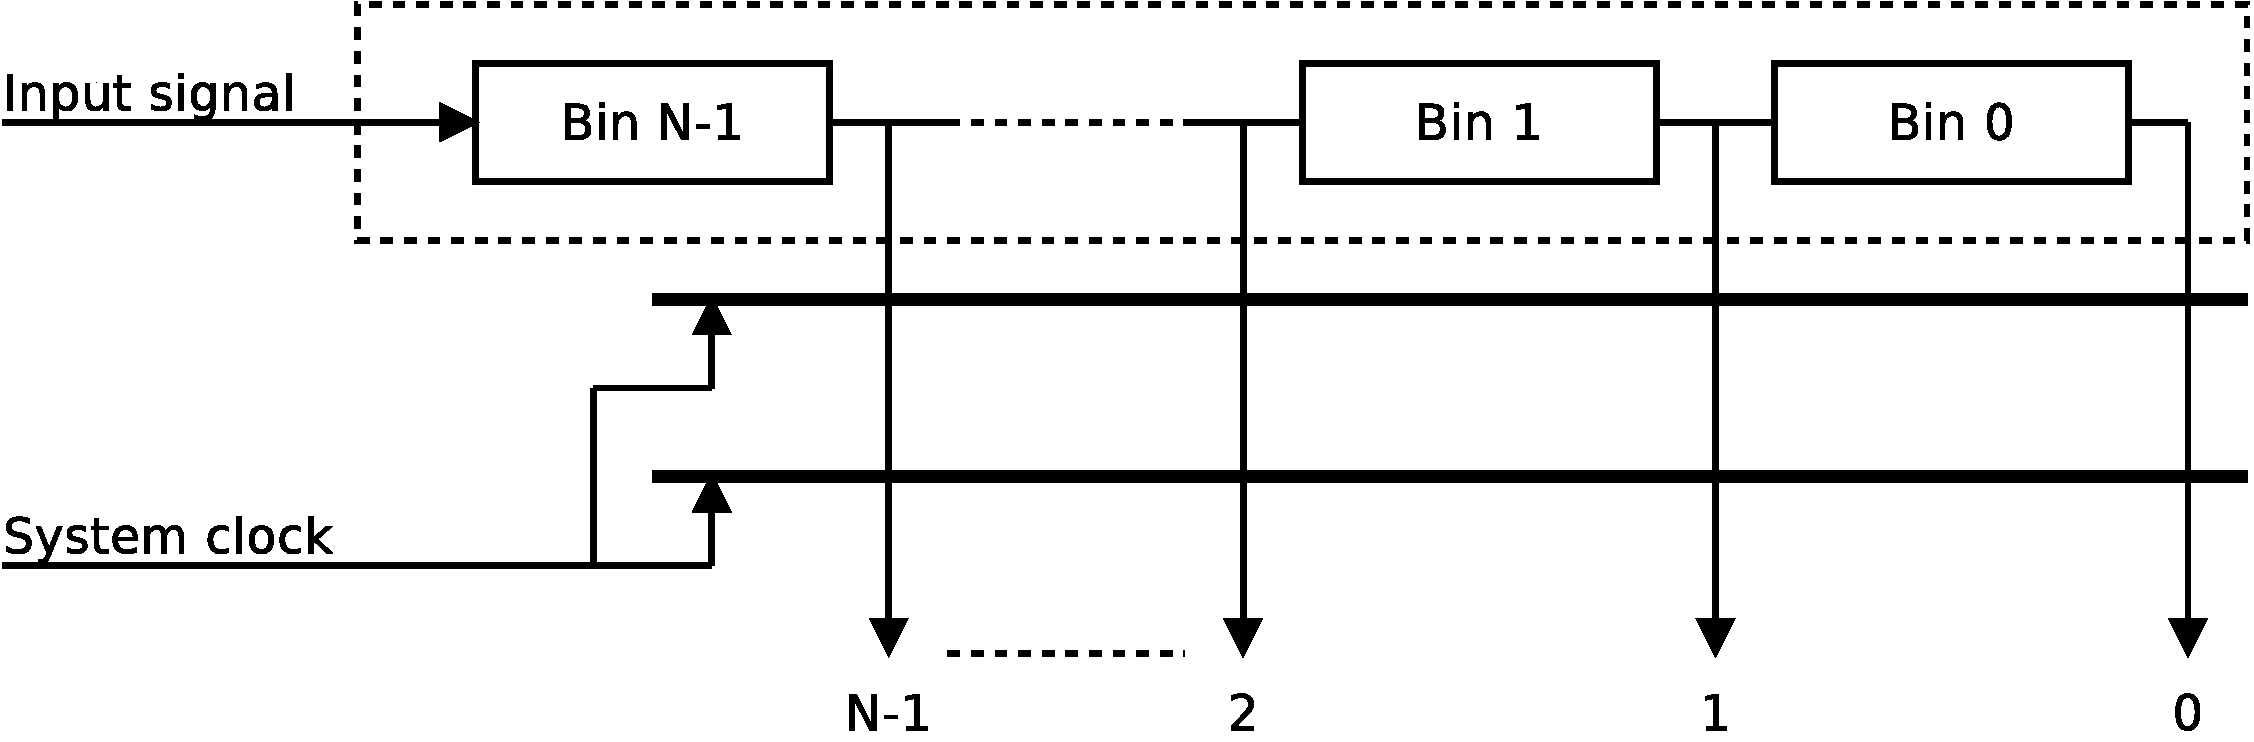
\includegraphics[width=\textwidth]{delaystruct.pdf}
\end{figure}

\section{Calibration mechanism}
In the formulas below:
\begin{itemize}
\item $T_{sys}$ is the system clock period.
\item $H(n)$ is the number of hits in the histogram at output $n$. A hit at output $n$ means that the signal propagated down to output $n$, without reaching output $n-1$.
\item $W(n)$ is the width of bin $n$.
\item $C = \displaystyle\sum\limits_{n=0}^{N-1} H(n)$ is the total number of hits in the histogram.
\item $R(n)$ is the time stamp of an event whose signal propagated down to output $n$ (without reaching output $n-1$), measured backwards from the clock tick.
\item $f$ (respectively $f_{0}$) is the current (respectively reference) frequency of the online calibration ring oscillator.
\end{itemize}

\subsection{Offline calibration}
\begin{equation}
W_{0}(N-1) = 0
\end{equation}
\begin{equation}
W_{0}(n) = \frac{H(n+1)}{C} \cdot T_{sys}
\end{equation}

\begin{equation}
R_{0}(n) = \displaystyle\sum\limits_{i=n}^{N-1}{W_{0}(i)} = \frac{T_{sys}}{C} \cdot \displaystyle\sum\limits_{i=n}^{N-1}{H(i)}
\end{equation}

\subsection{Online calibration}

\begin{equation}
R(n) = \frac{f_{0}}{f} \cdot R_{0}(n)
\end{equation}

\begin{thebibliography}{99}
\bibitem{s6hdl} Xilinx, \textsl{Spartan-6 Libraries Guide for HDL Designs}, \url{http://www.xilinx.com/support/documentation/sw_manuals/xilinx12_3/spartan6_hdl.pdf}
\bibitem{epfl} Claudio Favi and Edoardo Charbon, \textsl{A 17ps Time-to-Digital Converter Implemented in 65nm FPGA Technology}, ACM 2009, \url{http://infoscience.epfl.ch/record/139431}
\end{thebibliography}

\end{document}
